\section{\AlgName{} Algorithm}\label{sec:method}
The multi-fidelity optimization algorithm proposed in this paper relies on an iterative two-stage approach that maintains two separate surrogate models that share information between them. The first stage involves a search on a kriging based surrogate model for potential candidates, within a restricted region, to evaluate them using low-fidelity computations. The information from this search is used to update the first model and a co-kriging model that combines both low- and high-fidelity samples to approximate the high-fidelity objective function. In the second stage, a search is conducted using the co-kriging model to determine a suitable candidate for high-fidelity evaluation. These high-fidelity evaluations are used to update the co-kriging model and to determine the neighbourhood for the next search using the low-fidelity surrogate. The overarching framework is outlined in Algorithm~\ref{alg:main-alg}, followed by the discussion of its key components.  

\begin{algorithm}[h!]
\caption{\AlgName{} procedure}
\label{alg:main-alg}
\algsetup{linenosize=\footnotesize}
{\footnotesize 
\begin{algorithmic}[1]
\REQUIRE{$P$, problem data; $N_L$, max size of low-fidelity population; $T$, maximum number of evaluations; $\rho$, parameter set for LocalOCBA.}
\ENSURE{Best solution found $\V{x}^\beta$.}
\STATE{$X_v \ot LHS(P),\ \forall v \in \{L,H\}$} \COMMENT{Generate initial populations}
\STATE{$A_v,t \ot f_v(X_v,0),\ \forall v \in \{L,H\}$} \COMMENT{Evaluate initial populations}
\STATE{$\V{x}^\beta \ot \emptyset$} \COMMENT{Initialize $\V{x}^\beta$} 
\WHILE{$t < T$}
  \STATE{$M_L \ot Krige(A_L)$} \COMMENT{Update low-fidelity kriging model}
  \STATE{$M_C \ot CoKrige(A_L,A_H)$} \COMMENT{Update co-kriging model}
  \STATE{$\V{x} \ot GlobalSearch(M_C)$} \COMMENT{Globally search co-kriging model}
  \STATE{$\V{\alpha},t \ot f_H(\V{x},t)$} \COMMENT{Evaluate and update total cost}
  \STATE{$A_H \ot A_H \cup \{\V{\alpha}\}$} \COMMENT{Add $\V{\alpha}$ to high-fidelity archive}
  \STATE{$\V{x}^\beta \ot \min(f_H(\V{x}^\beta),f_H(\V{x}))$} \COMMENT{Update best solution}
  \STATE{$\epsilon \ot Sigmoid(t,T)$} \COMMENT{Determine size of neighbourhood}
  \STATE{$A_L,t \ot LocalOCBA(\rho,M_L,A_L,\V{x}^\beta,\epsilon)$} \COMMENT{Locally search low-fidelity model}
  \IF{$|A_L| > N_L$}
    \STATE{$A_L \ot Winnow(A_L,N_L)$} \COMMENT{Control population size}
  \ENDIF
\ENDWHILE
\end{algorithmic}
}
\end{algorithm}

\subsection{Initialization, evaluation and surrogate models}
The function $LHS(P)$ returns an initial population generated from a latin hypercube sampling~(LHS), the bounds of which are defined in $P$. LHS is used as it can provide well distributed solutions in the variable space without requiring exponential number of them, unlike full-factorial sampling. The solutions are evaluated using the function $f_v(X,t)$, at some fidelity $v\in \{L,H\}$, which returns a set of ``archive'' pairs comprising the solution and its objective value. It also updates the total cost incurred, $t$, taking into account the cost of evaluating the solutions at fidelity $v$. 

Two surrogate models are built: $Krige(A_L)$ takes the low-fidelity samples and returns a kriging model approximating it, and $CoKrige(A_L,A_H)$ takes both the low- and high-fidelity archive and returns a co-kriging model that approximates the fitness landscape of the high-fidelity objective function. The function $GlobalSearch(M_C)$ takes the co-kriging model as input and returns the best solution that can find using some global search method~(on the surrogate model). The solution identified from the above provcess is evaluated in high-fidelity and the information is used to update the co-kriging model, and also to determine the restricted neighbourhood to be used for search using the low-fidelity kriging model, discussed next.

\subsection{Restricted neighbourhood}\label{subsec:restrict}
The correlation between the low- and high-fidelity samples can vary significantly between problems, meaning identifying a promising region in the low-fidelity kriging model does not necessarily mean identifying a promising region in the high-fidelity co-kriging model. Therefore, instead of searching the low-fidelity model globally, it makes sense to search for promising candidates within a restricted neighbourhood, defined using information from the high-fidelity model. As the goal of performing low-fidelity evaluations in co-kriging models is to gain information about the shape of the fitness landscape, more than it is to find the ``best'' low-fidelity solution, restricting the neighbourhood in the algorithm to focus on the region of interest --- without getting ``distracted'' by global optima that might not be useful in the over-all search.

\ray{Angus can you please take stock of all symbols being used and see any double use. For example I see capitaal x in F(x) and also small bold}In order to restrict the region of interest, a so-called \emph{guided} differential evolution~(DE) process is employed. In DE, a candidate child solution $x_c$ is produced from three parent solutions $\V{x}^1$, $\V{x}^2$ and $\V{x}^3$ using the following formula~\cite{storn1997differential}:
\begin{equation}
\V{x}^c = \V{x}^1 + F(\V{x}^2 - \V{x}^3)\,,
\end{equation}
where $F$ is a constant called the mutation factor. This can also be thought of as scaled vector addition, therefore it is possible to direct the resulting child $\V{x}^c$ towards a reference point~(say $\V{x}^\beta$) by adjusting the mutation in the following way:
\begin{equation}\label{eq:nudge}
\V{x}^{c'} = \V{x}^c + \V{g}\cdot(\V{x}^\beta - \V{x}^c)\,,
\end{equation}
where $\V{g}$ is the so-called \emph{guide factor}. This is illustrated in Figure~\ref{fig:guide-DE}. \hemant{The factor $G$ should be a scalar, therefore I've removed its bold font.}\angus{see below}

\begin{figure}[h!]
\centering
\adjustbox{max width=0.5\textwidth}{%
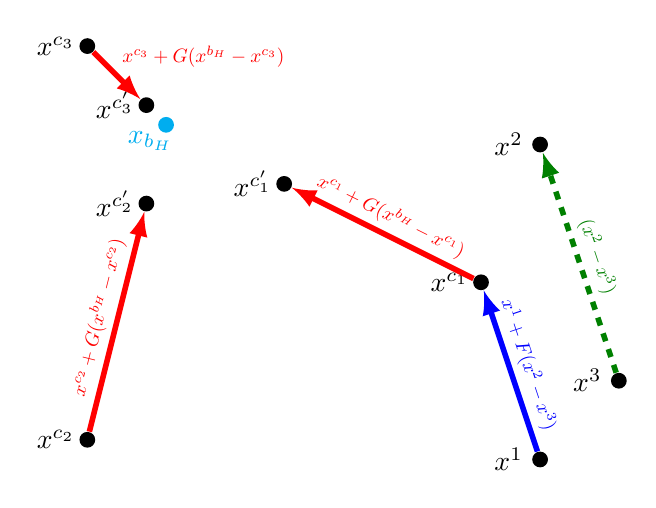
\begin{tikzpicture}

\node [fill, circle,inner sep=0pt,minimum size=2mm] (x1) at (0,0) {};
\node [fill, circle,inner sep=0pt,minimum size=2mm] (x3) at (1,1) {};
\node [fill, circle,inner sep=0pt,minimum size=2mm] (x2) at (0,4) {};
\node [fill, circle,inner sep=0pt,minimum size=2mm] (xc1) at (-0.75,2.25) {};
\node [fill, circle,inner sep=0pt,minimum size=2mm,color=cyan] (xb) at (-4.75,4.25) {};
\node [fill, circle,inner sep=0pt,minimum size=2mm] (xc1p) at (-3.25,3.5) {};
\node [fill, circle,inner sep=0pt,minimum size=2mm] (xc2) at (-5.75,0.25) {};
\node [fill, circle,inner sep=0pt,minimum size=2mm] (xc2p) at (-5,3.25) {};
\node [fill, circle,inner sep=0pt,minimum size=2mm] (xc3) at (-5.75,5.25) {};
\node [fill, circle,inner sep=0pt,minimum size=2mm] (xc3p) at (-5,4.5) {};

\node [xshift = -4mm] (x1t) at (x1) {$\V{x}^1$};
\node [xshift = -4mm] (x2t) at (x2) {$\V{x}^2$};
\node [xshift = -4mm] (x3t) at (x3) {$\V{x}^3$};
\node [xshift = -4mm] (xc1t) at (xc1) {$\V{x}^{c_1}$};
\node [xshift = -4mm] (xc2t) at (xc2) {$\V{x}^{c_2}$};
\node [xshift = -4mm] (xc3t) at (xc3) {$\V{x}^{c_3}$};
\node [xshift = -2mm,yshift = -2mm,color=cyan] (xbt) at (xb) {$x_{b_H}$};
\node [xshift = -4mm] (xc1pt) at (xc1p) {$\V{x}^{c_1'}$};
\node [xshift = -4mm] (xc2pt) at (xc2p) {$\V{x}^{c_2'}$};
\node [xshift = -4mm] (xc3pt) at (xc3p) {$\V{x}^{c_3'}$};

\draw [-latex,line width=2,color=Green,dashed] (x3) -- node[sloped,above,scale=0.7] {$(\V{x}^2-\V{x}^3)$} (x2);
\draw [-latex,line width=2,color=Blue] (x1) -- node[sloped,above,scale=0.7] {$\V{x}^1+F(\V{x}^2-\V{x}^3)$} (xc1);
\draw [-latex,line width=2,color=Red] (xc1) -- node[sloped,above,scale=0.7] {$\V{x}^{c_1}+G(\V{x}^{b_H}-\V{x}^{c_1})$} (xc1p);
\draw [-latex,line width=2,color=Red] (xc2) -- node[sloped,above,scale=0.7] {$\V{x}^{c_2}+G(\V{x}^{b_H}-\V{x}^{c_2})$} (xc2p);
\draw [-latex,line width=2,color=Red] (xc3) -- node[xshift=11mm,above,scale=0.7] {$\V{x}^{c_3}+G(\V{x}^{b_H}-\V{x}^{c_3})$} (xc3p);

\end{tikzpicture}
}
\caption{The DE recombination process can be ``guided'' towards the best high-fidelity solution found so far.}\label{fig:guide-DE}
\end{figure}

In this figure, it can be seen that $\V{x}^{c_1}$ is produced using $\V{x}^1$, $\V{x}^2$ and $\V{x}^3$, and then translated using Equation~\ref{eq:nudge} to produce $\V{x}^{c_1'}$. Child solutions $\V{x}^{c_2}$ and $\V{x}^{c_3}$ are produced using two other sets of solutions that are not pictured, and then translated using the same equation. If this process is continued, the result is a cloud of candidate solutions in the vicinity of $\V{x}^\beta$, the centre of the region of interest.

The guide factor is a vector, each component of which determines how far the resulting solution is attracted to $\V{x}^\beta$ in a given direction. At the beginning of the search, $\V{x}^\beta$ is determined by optimising a very coarse model built with sparse information, and cannot be trusted to be indicative of a promising region of the search space. As the search continues, the model becomes more accurate and the information it produces more trustworthy. Therefore, the algorithm should be explorative in the beginning of the search, but exploitative towards the end. One function which exhibits these properties is the logistic sigmoid curve:
\begin{equation}
\epsilon = \dfrac{L}{1+e^{-k(x-x_0)}}\,,
\end{equation}
where $x_0$ is the $x$ value of the sigmoid's midpoint, $L$ is the curve's maximum and $k$ is the steepness parameter, which controls how fast the function rises. The function $Sigmoid(t,T)$ uses the total cost and maximum cost to compute this $\epsilon$ value. Figure~\ref{fig:logistic} gives a plot of the logistic sigmoid curve with $L=0.99$, $k=10$ and $x_0 = 0.2$. 
\begin{figure}[h!]
  \centering
  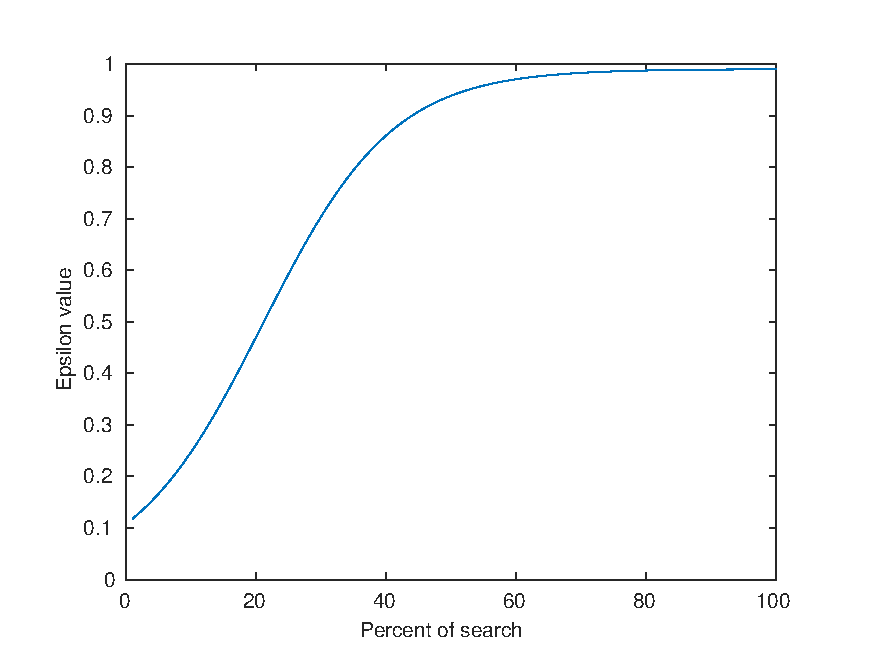
\includegraphics[width = 0.40\textwidth]{img/logistic.eps} 
  \caption{The logistic sigmoid curve flattens at around 80\%.} 
    \label{fig:logistic}
\end{figure}
Using this value, $\V{g}$ can be computed as:
\begin{equation}
\V{g} = \epsilon + (1-\epsilon)\V{r}\,,
\end{equation}
where $\V{r} \in [0,1]^D$ is a random vector with $D$ components, making $\V{g} \in [\epsilon,1]^D$ also a random vector. \hemant{Equation~13 appears misleading to me; it could just be a notation issue. Basically, the vectors in the $\V{x}$ space get mixed up with the mention of vectors $\V{g}$ and $\V{r}$. It might be easier to present $g$~(should be $G$ I think) and $r$ simply as a scalars, and say that you use the equation for generating each solution $r$ sampled from a uniform random distribution.}\angus{you're right that there was some notation mix-up between $\V{G}$ and $\V{g}$, so i fixed that. However, $\V{g}$ is not a scalar, it is a vector where each element of the vector influences how much the new solution is attracted to the best solution so far, in a given direciton. I have updated the text above to clarify that. I initially made it a scalar, but it seemed to work better allowing each direction to scale differently. I think having the only possible solutions lying on the $\V{x}^\beta - \V{x}$ line was too greedy, especially later in the search. Allowing $\V{g}$ to be a vector means the new solution can be anywhere in a quadrant region with a diagonal from $\V{x}^\beta$ to $\epsilon(\V{x}^\beta - \V{x})$.. Looking at the diagram, i realise that it does look like $\V{g}$ is a scalar, as the translations are all explicitly in the $\V{x}^\beta - \V{x}$ direction, so i will think about how to represent it better --- maybe shaded regions for the possible values might work..} This ensures the cloud of candidate solutions around $\V{x}^\beta$ is sparse at the beginning of the search, allowing for better global exploration, while focusing the search more tightly on promising regions towards the end. Crucially, the parameters needed to control the sigmoid curve are intuitive to set and do not require tuning to achieve the desired behavior.

\subsection{LocalOCBA}\label{subsec:local}
Once the candidate solutions have been been generated in the vicinity of $\V{x}^\beta$, some of them need to be selected for evaluation at low-fidelity. As already stated, the goal of evaluating solutions in low-fidelity is not to optimize the low-fidelity objective function, but to provide as much information for the model as possible. The optimal computing budget allocation (OCBA) algorithm selects from a set of solutions with the goal of reducing uncertainty within simulation models by adaptively allocating computing resources. This principle can be applied here, with some modifications, as outlined in Algorithm~\ref{alg:local-ocba}.

\begin{algorithm}[h!] 
\caption{$LocalOCBA$ procedure}
\label{alg:local-ocba}
\algsetup{linenosize=\footnotesize}
{\footnotesize
\begin{algorithmic}[1]
\REQUIRE{$\rho=\{\Delta_1$, total to be sampled; $\Delta_2$, samples per statistics update$\}$; $M$, low-fidelity model; $A_L$, low-fidelity archive; $\V{x}^\beta$, best high-fidelity solution ; $\epsilon$, sigmoid value; $t$, total cost incurred.}
\ENSURE{$A_L$, updated low-fidelity archive; $t$, updated total cost.}
\STATE{$X \ot GuidedDE(A_L,\V{x}^\beta,\epsilon)$} \COMMENT{Generate child population}
\STATE{$A_X \ot f_{M}(X)$} \COMMENT{Approximate each child by model $M$}
\STATE{$G,q \ot Partition(A_X)$} \COMMENT{Partition solutions}
\STATE{$S_i \ot \emptyset,\ \forall i \in [q]$} \COMMENT{Empty groups for selected solutions}
\WHILE{$\displaystyle\sum_{i \in [q]} |S_i| < \Delta_1$}\label{while-loop}
  \STATE{$\hat{\mu}_i,\hat{\sigma}_i \ot$ sample statistics for $S_i$, $\forall i \in [q]$ (if $|S_i| < 2$, use $G_i$)}
  \STATE{$R \ot GetRatios(\V{\hat{\mu}},\V{\hat{\sigma}})$} \COMMENT{compute allocation ratios}
  \STATE{$D \ot Allocate(R,S,G) : \displaystyle\sum_{i \in [q]}|D_i| = \Delta_2$} \COMMENT{Allocate $\Delta_2$ solutions according to ratios $R$}
  \STATE{$D_i,t \ot f_L(D_i,t),\ \forall i \in [q]$} \COMMENT{Evaluate allocated solutions}
  \STATE{$S_i \ot S_i \cup D_i,\ \forall i \in [q]$} \COMMENT{Add to selected solutions}
  \STATE{$G_i \ot G_i \setminus D_i,\ \forall i \in [q]$} \COMMENT{Selection without replacement}
\ENDWHILE
\STATE{$A_L \ot A_L \cup \displaystyle\bigcup_{i \in [q]} S_i$} \COMMENT{Combine all selected solutions}
\end{algorithmic}
}
\end{algorithm}

Here, the $GuidedDE(A_L,\V{x}^\beta,\epsilon)$ process is used to generate a set of candidate solutions, which are approximated using $f_M(X)$. This function takes a set of solutions and returns a set of pairs comprising the solution and its approximation on the (surrogate) model $M$. The solutions are ranked and partitioned using a $k$-means clustering algorithm, based on their approximated value. The purpose of ranking the solutions first is to increase the probability that solutions within a clustered group will tend to have a similar performance to each other, regardless of their proximity in the decision space. This helps to ensure diversity of selected solutions, while still preferring the more promising candidates. The function $Partition(X)$ returns a set of solution groups $G$ and the number of groups $q$.

OCBA principles are used to select --- and remove --- from these groups to populate a set of empty groups $S$. First, sample statistics are computed for all groups of selected solutions in $S$. If there are fewer than two solutions in a group, then its corresponding group in $G$ is used. The function $GetRatios(\V{\hat{\mu}},\V{\hat{\sigma}})$ uses these statistics to compute allocation ratios in accordance for each group with standard OCBA practice. These ratios are used by $Allocate(R,S,G)$ to allocate $\Delta_2$ solutions to be evaluated as low-fidelity and added to the selected solutions $S$.

Once $\Delta_1$ solutions have been selected in the set $S$, they are evaluated in the low-fidelity. Then, they are added to the low-fidelity archive, and the updated archive is returned.

\subsection{Archive size control}
Due to the fact that many more low-fidelity solutions are added to the archive between each high-fidelity evaluation, the size of the low-fidelity archive can become too big for some kriging and co-kriging algorithms, or too concentrated if the search is focused on the same area for too long. Therefore, a maximum archive size $N_L$ is set such that once it reaches that threshold, the population should be maintained at that level. Choosing a steady-state method such as ranking the solutions by their value and selecting the top $N_L$ will cause the population to converge and lose diversity over time. As the purpose of maintaining the low-fidelity population is to provide the co-kriging model with information about the shape of the fitness landscape, this loss of diversity can be detrimental. 

The function $Winnow(A_L,N_L)$ processes an archive of solutions and returns a winnowed archive with exactly $N_L$ solutions. It does this by partitioning the solutions in the decision space into $N_L$ different groups using a clustering algorithm, such as $k$-means clustering. Most of these clusters will contain only one solution which are directly added to the winnowed archive; for those that have more than one solution, only the solution with the best value is selected. This ensures that the archive never has more than $N_L$ solutions, but diversity is maintained throughout the population.

\subsection{Similarities and differences to \motos{}}
There exist some similarities between \AlgName{} and the \motos{} framework. For example, both use a two-step process of ordering a population of solutions and then selecting from them using ideas from OCBA. Despite the similarities, there are several key aspects which differentiate the two algorithms from each other. 

The biggest difference is that \AlgName{} involves an iterative sampling and evaluation process, whereas \motos{} is a two-step algorithm which is only executed once. As \motos{} only performs a single iteration, it is not able to use any prior knowledge to dynamically determine where it should concentrate its resources when evaluating the initial low-fidelity population. Therefore, it evaluates uniformly across the whole search space, and subsequently spends computational budget in areas which are not beneficial to the search. In contrast, \AlgName{} uses information from previous iterations, to identify promising areas of the search space that it can exploit.

Another difference is that \motos{} operates on the high- and low-fidelity objective functions directly across the entire search space. Solutions are selected using information from low-fidelity evaluations, to be evaluated in high-fidelity. In contrast, \AlgName{} uses its ranking and selection phases in order to select from a neighbourhood of solutions that have been identified as promising regions of the search space. These selections are informed by a kriging model of the low-fidelity function, and selected for low-fidelity evaluation. The high-fidelity evaluations are determined by a separate search that is performed on the co-kriging model, updated by the selected low-fidelity evaluations. Because of this, it is not necessary to perform the initial $n_0$ evaluations before computing the sample statistics, as the goal is not to optimize the low-fidelity objective function but rather just select from a set of ranked candidates.

The fact that \motos{} must determine all of its candidates \emph{a priori} means that it can only sample from a pre-defined, finite set of solutions, and is unable to refine what it produces. To achieve a high precision, a large number of low-fidelity evaluations solutions may be required. Since low-fidelity evaluations have low but non-zero cost in relation to high-fidelity, the computational effort required in sampling large set of solutions in low-fidelity can still be excessive. This is illustrated in Figure~\ref{fig:motos-example}. By doing on-line sampling and creating a surrogate model which can be used for global search, \AlgName{} is, in theory, able to produce any feasible solution in the search space and improve upon the promising candidates by focusing the search on their local neighbourhood.

Finally, \motos{} partitions the ranked population into a fixed number of equal-sized groups, whereas \AlgName{} uses a clustering algorithm to determine the number and size of partitions. This ensures that the average distance between groups in objective space is maximized. %\hemant{Referring back to my comment in the previous section, here is where you can revisit/redraw the figure and show how the next selected point(s) are of higher quality for your algorithm. Of course it will not demonstrate every component of your algorithm, but at least the concept demonstration why your selection method is likely to improve performance.}

\subsection{Proof of concept}
To visualise the operation of the proposed method and demonstrate its advantages, \AlgName{} is applied to the motivating example given in Section~\ref{sec:back} with a limited computational budget (200 low-fidelity-equivalent evaluations) to highlight the shortcomings of the \motos{} algorithm (Figure~\ref{fig:ex-mfits}).
\begin{figure*}[t]
  \centering
  \subfloat[105 unit cost, $x^\beta = -1.4202$\label{fig:ex-mfits105}]{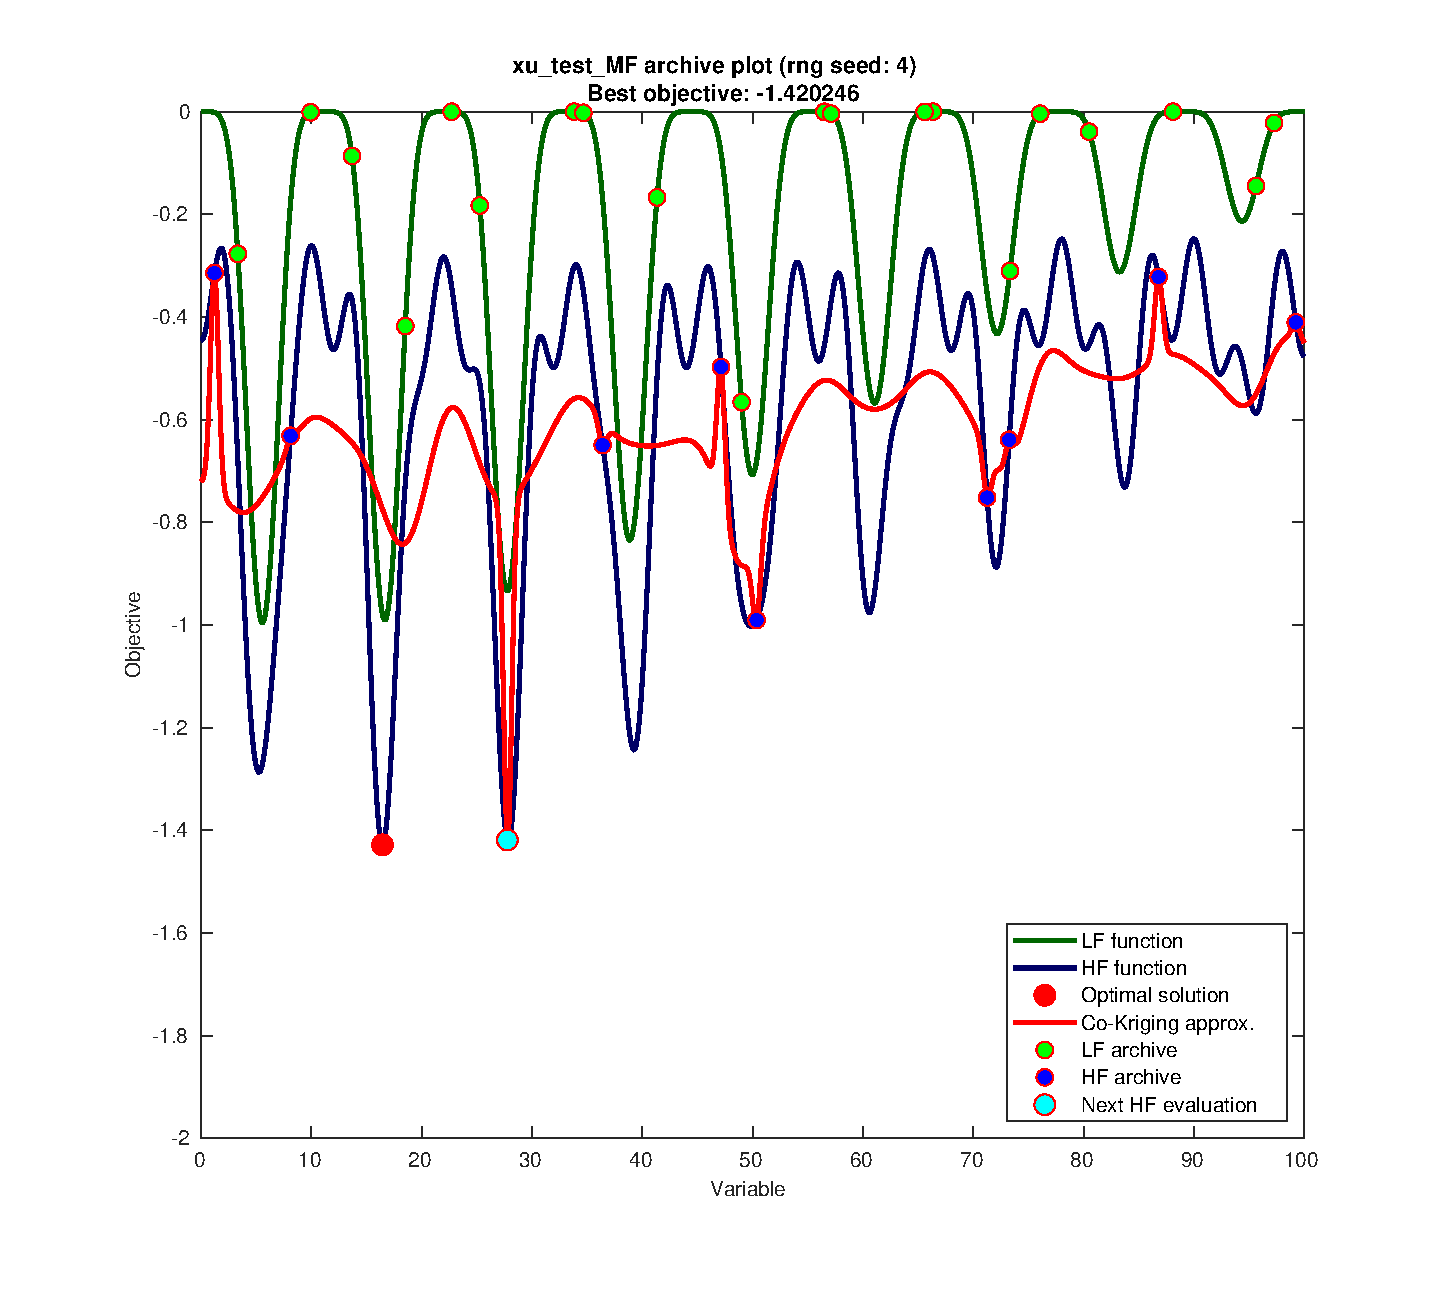
\includegraphics[width = 0.25\textwidth]{img/ex_mfits_01.eps}} 
  \subfloat[134 unit cost, $x^\beta = -1.4221$\label{fig:ex-mfits134}]{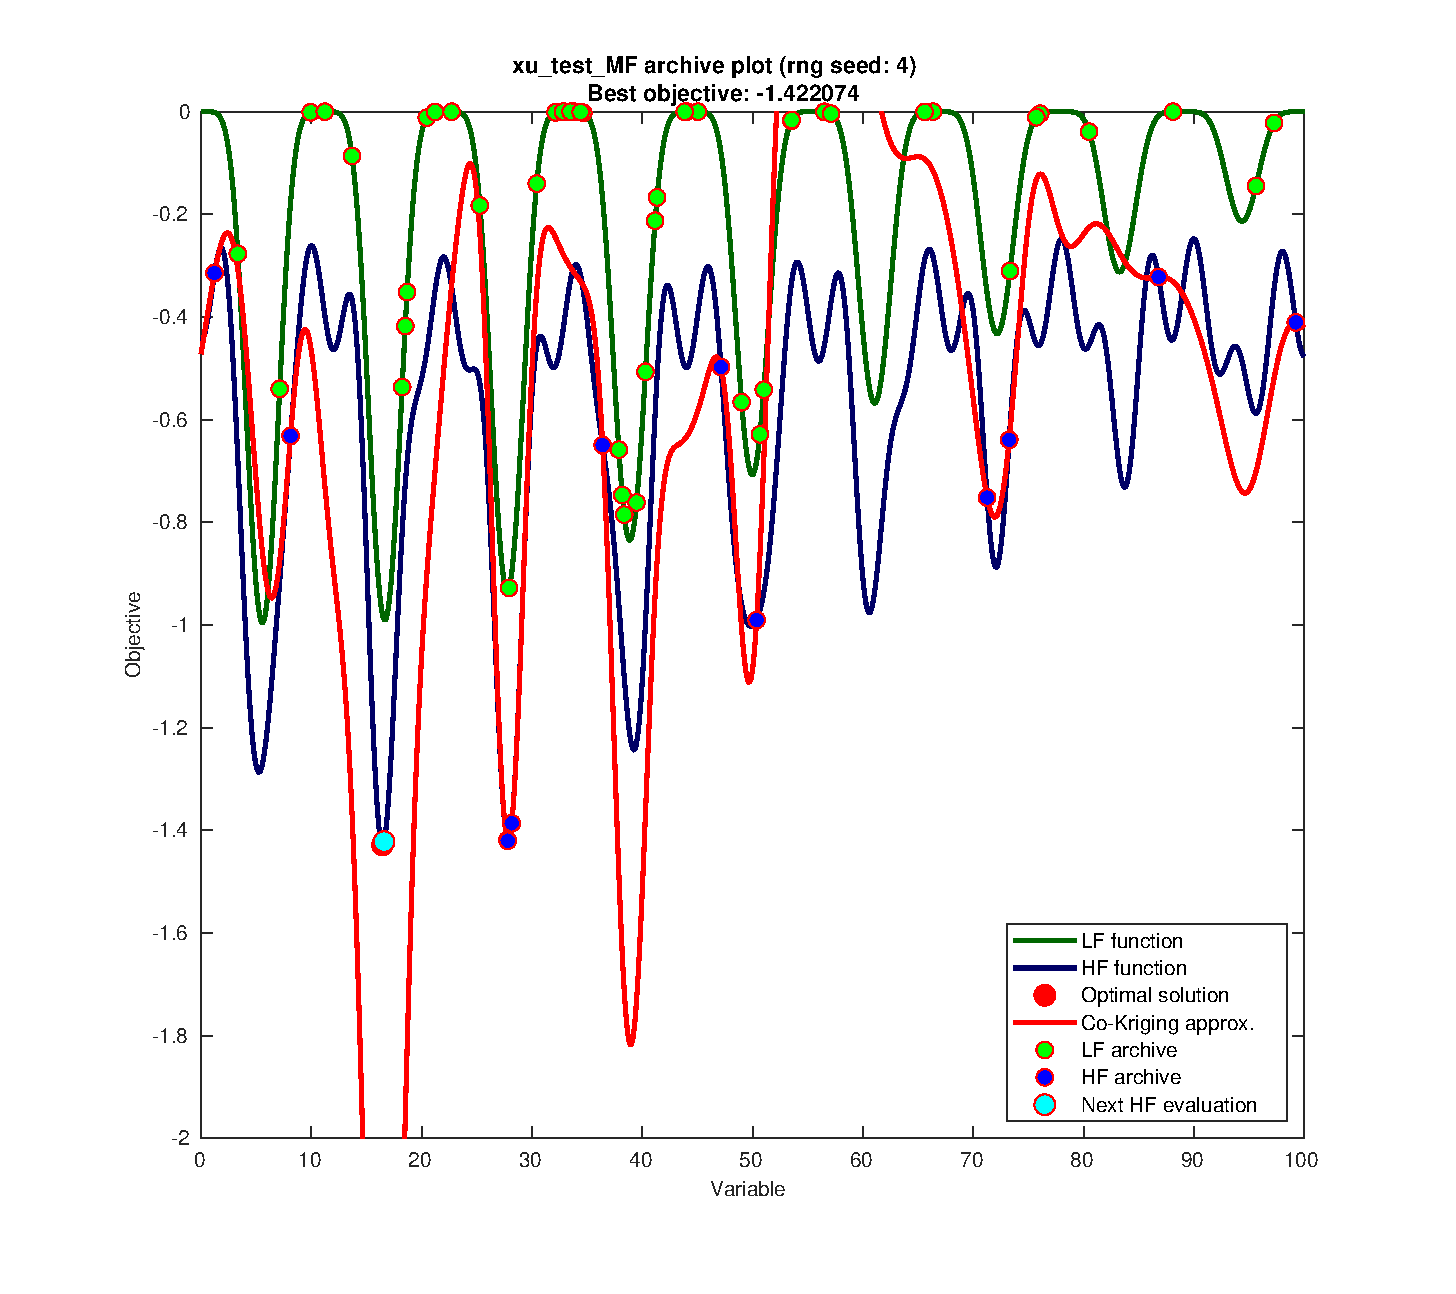
\includegraphics[width = 0.25\textwidth]{img/ex_mfits_04.eps}} 
  \subfloat[167 unit cost, $x^\beta = -1.4221$\label{fig:ex-mfits167}]{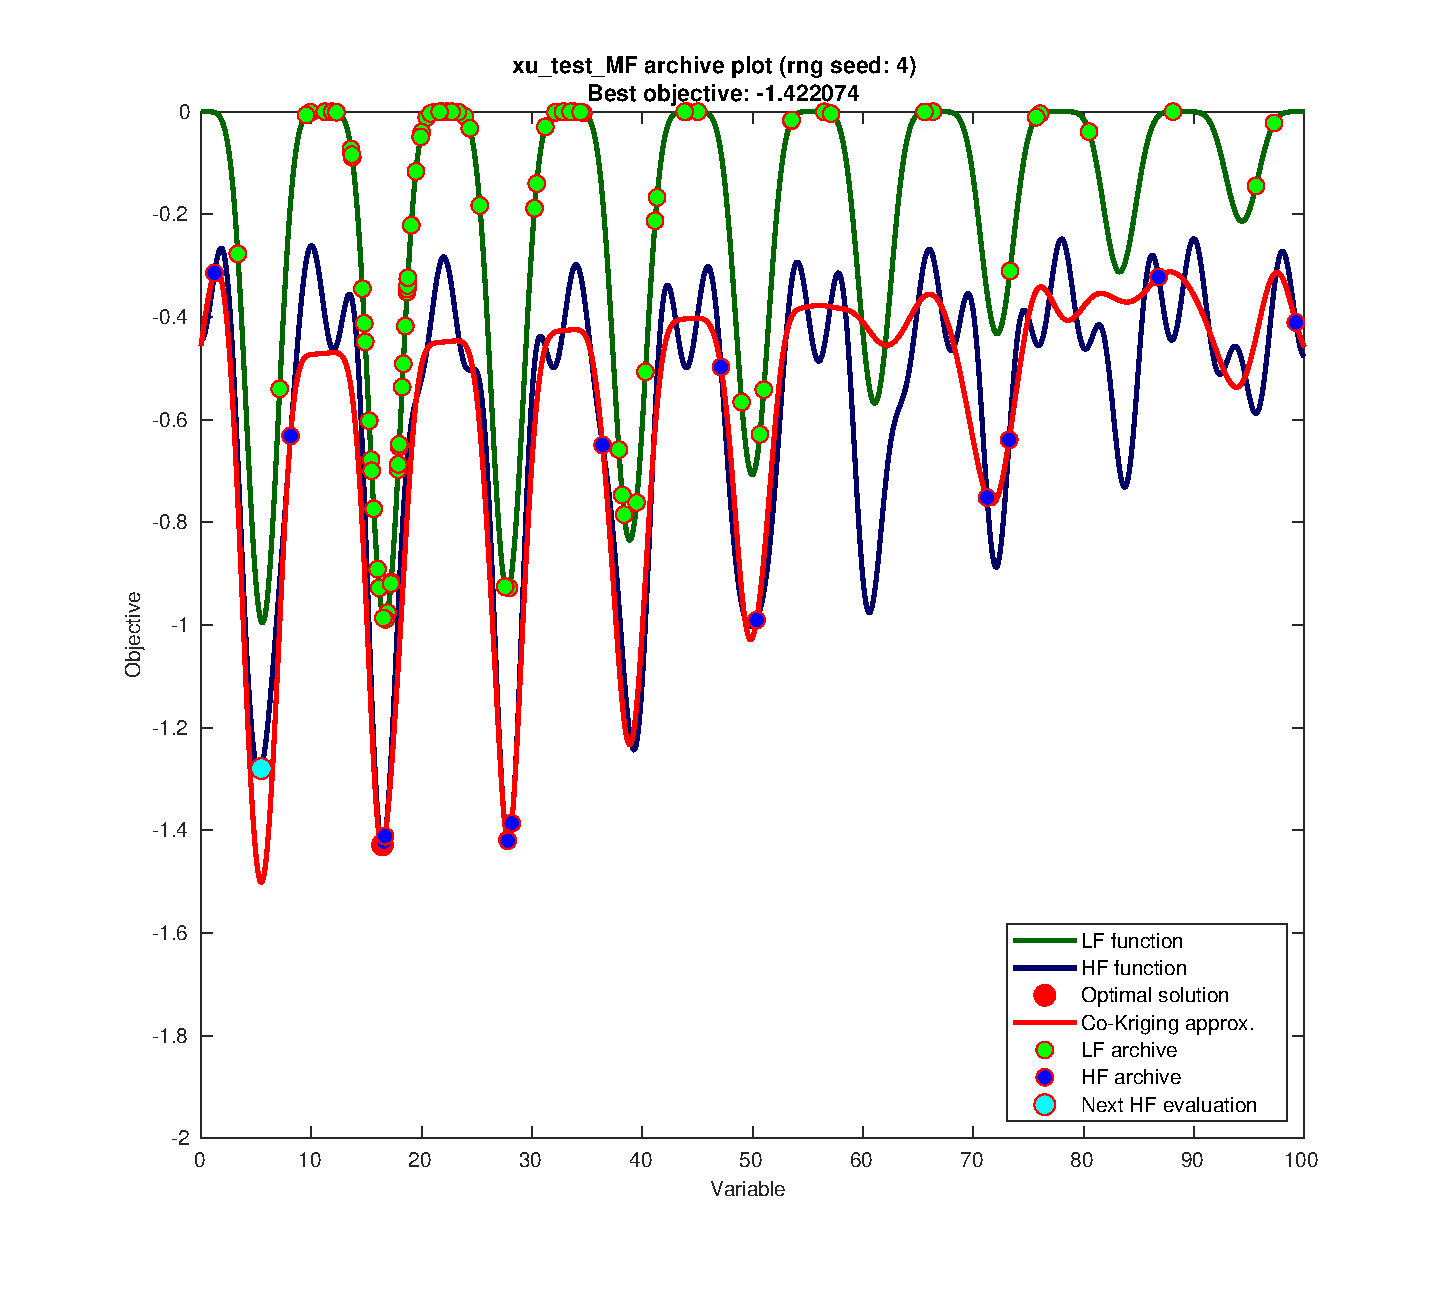
\includegraphics[width = 0.25\textwidth]{img/ex_mfits_06.eps}}
  \subfloat[200 unit cost, $x^\beta = -1.4281$\label{fig:ex-mfits200}]{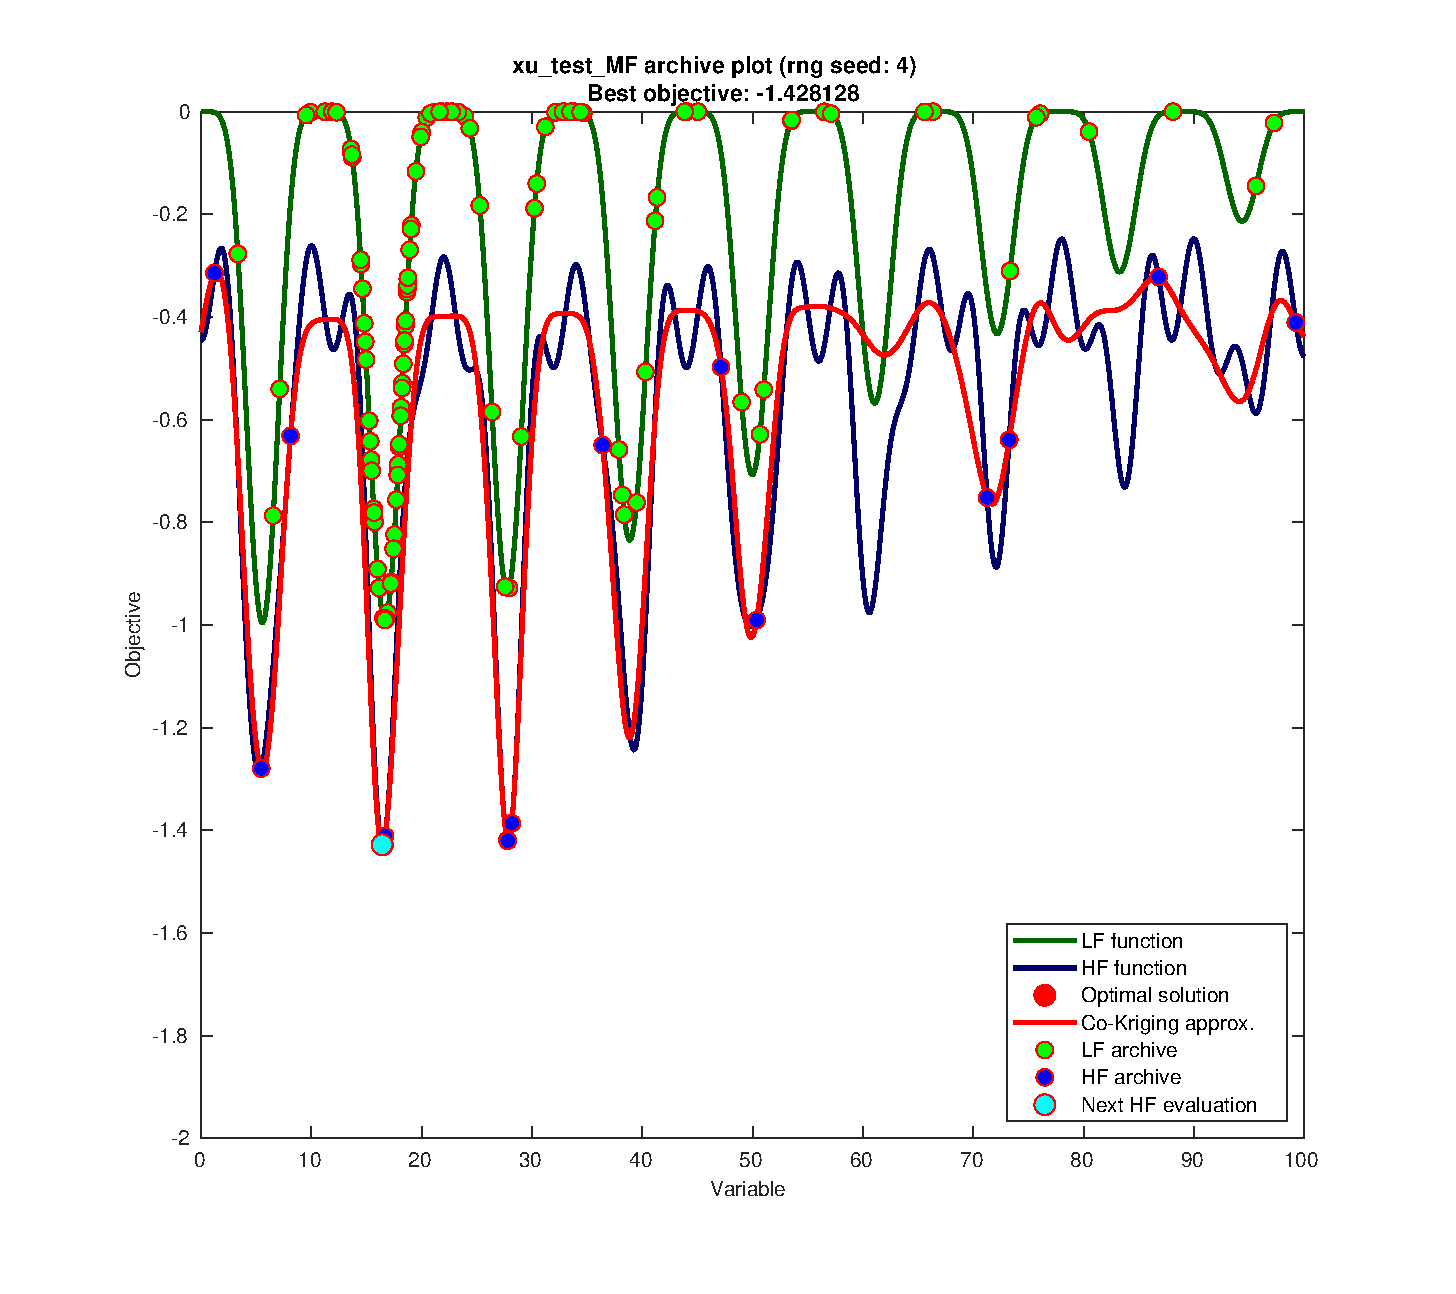
\includegraphics[width = 0.25\textwidth]{img/ex_mfits_07.eps}}
  \caption{Snapshot of \AlgName{} applied to Equations~\ref{eq:hf-ex} and~\ref{eq:lf-ex}, with corresponding budget consumed and best solution, $x^\beta$.} 
    \label{fig:ex-mfits}
\end{figure*}
\ray{same comment as earlier for these plots too}In this figure, the green and blue lines are the low- and high-fidelity response surfaces, respectively; the red line is the co-kriging approximation of the high-fidelity function, green and blue points represent the low- and high-fidelity archives, respectively; the cyan point is the next solution chosen for high-fidelity evaluation; and the red point is the optimal solution, $\V{x}^*$. Each sub-figure gives a snapshot of the operation of \AlgName{} on this example, for a given unit cost.

Initially (Figure~\ref{fig:ex-mfits105}), the co-kriging approximation is poor, as there are very few samples to inform it and the global search on this model selects a candidate for high-fidelity evaluation which is in the valley adjacent to the one which contains $\V{x}^*$. The search remains in this valley, until the co-kriging model has gathered enough information about the landscape to escape the local optima (Figure~\ref{fig:ex-mfits134}), where the global search selects a solution that is closer to optimal. In evaluating this new solution, the model is updated again such that it selects a candidate in the valley to the left of the optimal solution (Figure~\ref{fig:ex-mfits167}), which has a worse objective than the current best when evaluated. Finally, there is one more update (Figure~\ref{fig:ex-mfits200}) which results in the final high-fidelity evaluation of -1.4281, which is near optimal. Xu et al. report the ``optimum'' as -1.4277, a result of their descretization of the search space, meaning \motos{} was not able to find the optimum due to precision issues.

Something also to note about Figure~\ref{fig:ex-mfits200} is the concentration of the low-fidelity samples on the left, an evidence that the guided DE process is using the computational budget efficiently, focusing only in the areas of the search it has identified as promising. The No Free Lunch Theorem~\cite{wolpert1997no} says there must be a trade-off for this concentration --- and lack --- of attention in certain regions, meaning that the co-kriging approximation is much poorer on the right-hand side of the plot than the left. However, this does not affect the search negatively as the quality of solutions in this region is poor as well.